\documentclass[10pt,twocolumn,letterpaper]{article}

\usepackage{iccv}
\usepackage{times}
\usepackage{epsfig}
\usepackage{graphicx}
\usepackage{amsmath}
\usepackage{amssymb}
\usepackage{makecell}
\usepackage[ruled,vlined,linesnumbered]{algorithm2e}
%\usepackage{algpseudocode}% http://ctan.org/pkg/algorithmicx
%usepackage{pbox}
%\usepackage[export]{adjustbox}
\newcommand\floor[1]{\lfloor#1\rfloor}
\newcommand\ceil[1]{\lceil#1\rceil}
\usepackage{subfig}
\usepackage[utf8]{inputenc}
\usepackage{array}
\newcolumntype{C}[1]{>{\centering\let\newline\\\arraybackslash\hspace{0pt}}m{#1}}
% I
% Include other packages here, before hyperref.

% If you comment hyperref and then uncomment it, you should delete
% egpaper.aux before re-running latex.  (Or just hit 'q' on the first latex
% run, let it finish, and you should be clear).
\usepackage[pagebackref=true,breaklinks=true,letterpaper=true,colorlinks,bookmarks=false]{hyperref}

% \iccvfinalcopy % *** Uncomment this line for the final submission

\def\iccvPaperID{244} % *** Enter the ICCV Paper ID here
\def\httilde{\mbox{\tt\raisebox{-.5ex}{\symbol{126}}}}

% Pages are numbered in submission mode, and unnumbered in camera-ready
\ificcvfinal\pagestyle{empty}\fi
\begin{document}

%%%%%%%%% TITLE
\title{Personalized Image Aesthetics}

\author{First Author\\
Institution1\\
Institution1 address\\
{\tt\small firstauthor@i1.org}
% For a paper whose authors are all at the same institution,
% omit the following lines up until the closing ``}''.
% Additional authors and addresses can be added with ``\and'',
% just like the second author.
% To save space, use either the email address or home page, not both
\and
Second Author\\
Institution2\\
First line of institution2 address\\
{\tt\small secondauthor@i2.org}
}

\maketitle
%\thispagestyle{empty}

\begingroup
\let\clearpage\relax
%****************************************************************
%*************abstract*******************************************

\begin{abstract}
Automatic image aesthetics rating has received a growing interest with the recent breakthrough in deep learning. Although many studies exist for learning a generic or universal aesthetics model, investigation of aesthetics models incorporating individual user's preference is quite limited. 
We address this personalized aesthetics problem by showing that individual's aesthetic preferences exhibit strong correlations with content and aesthetic attributes, and hence the deviation of individual's perception from generic image aesthetics is predictable. 
To accommodate our study, we first collect two distinct datasets, a large image dataset from Flickr and annotated by Amazon Mechanical Turk, and a small dataset of real personal albums rated by owners. We then propose a new approach to personalized aesthetics learning that can be trained even with a small set of annotated images from a user. The approach is based on a residual-based model adaptation scheme which learns an offset to compensate for the generic aesthetics score. Finally, we introduce an active learning algorithm to optimize personalized aesthetics prediction for real-world application scenarios. Experiments demonstrate that our approach can effectively learn personalized aesthetics preferences, and outperforms existing methods on quantitative comparisons. 

\end{abstract}

%****************************************************************
%***************introduction****************************************
%****************figure: demo user-specific************************
\begin{figure}
\begin{center}
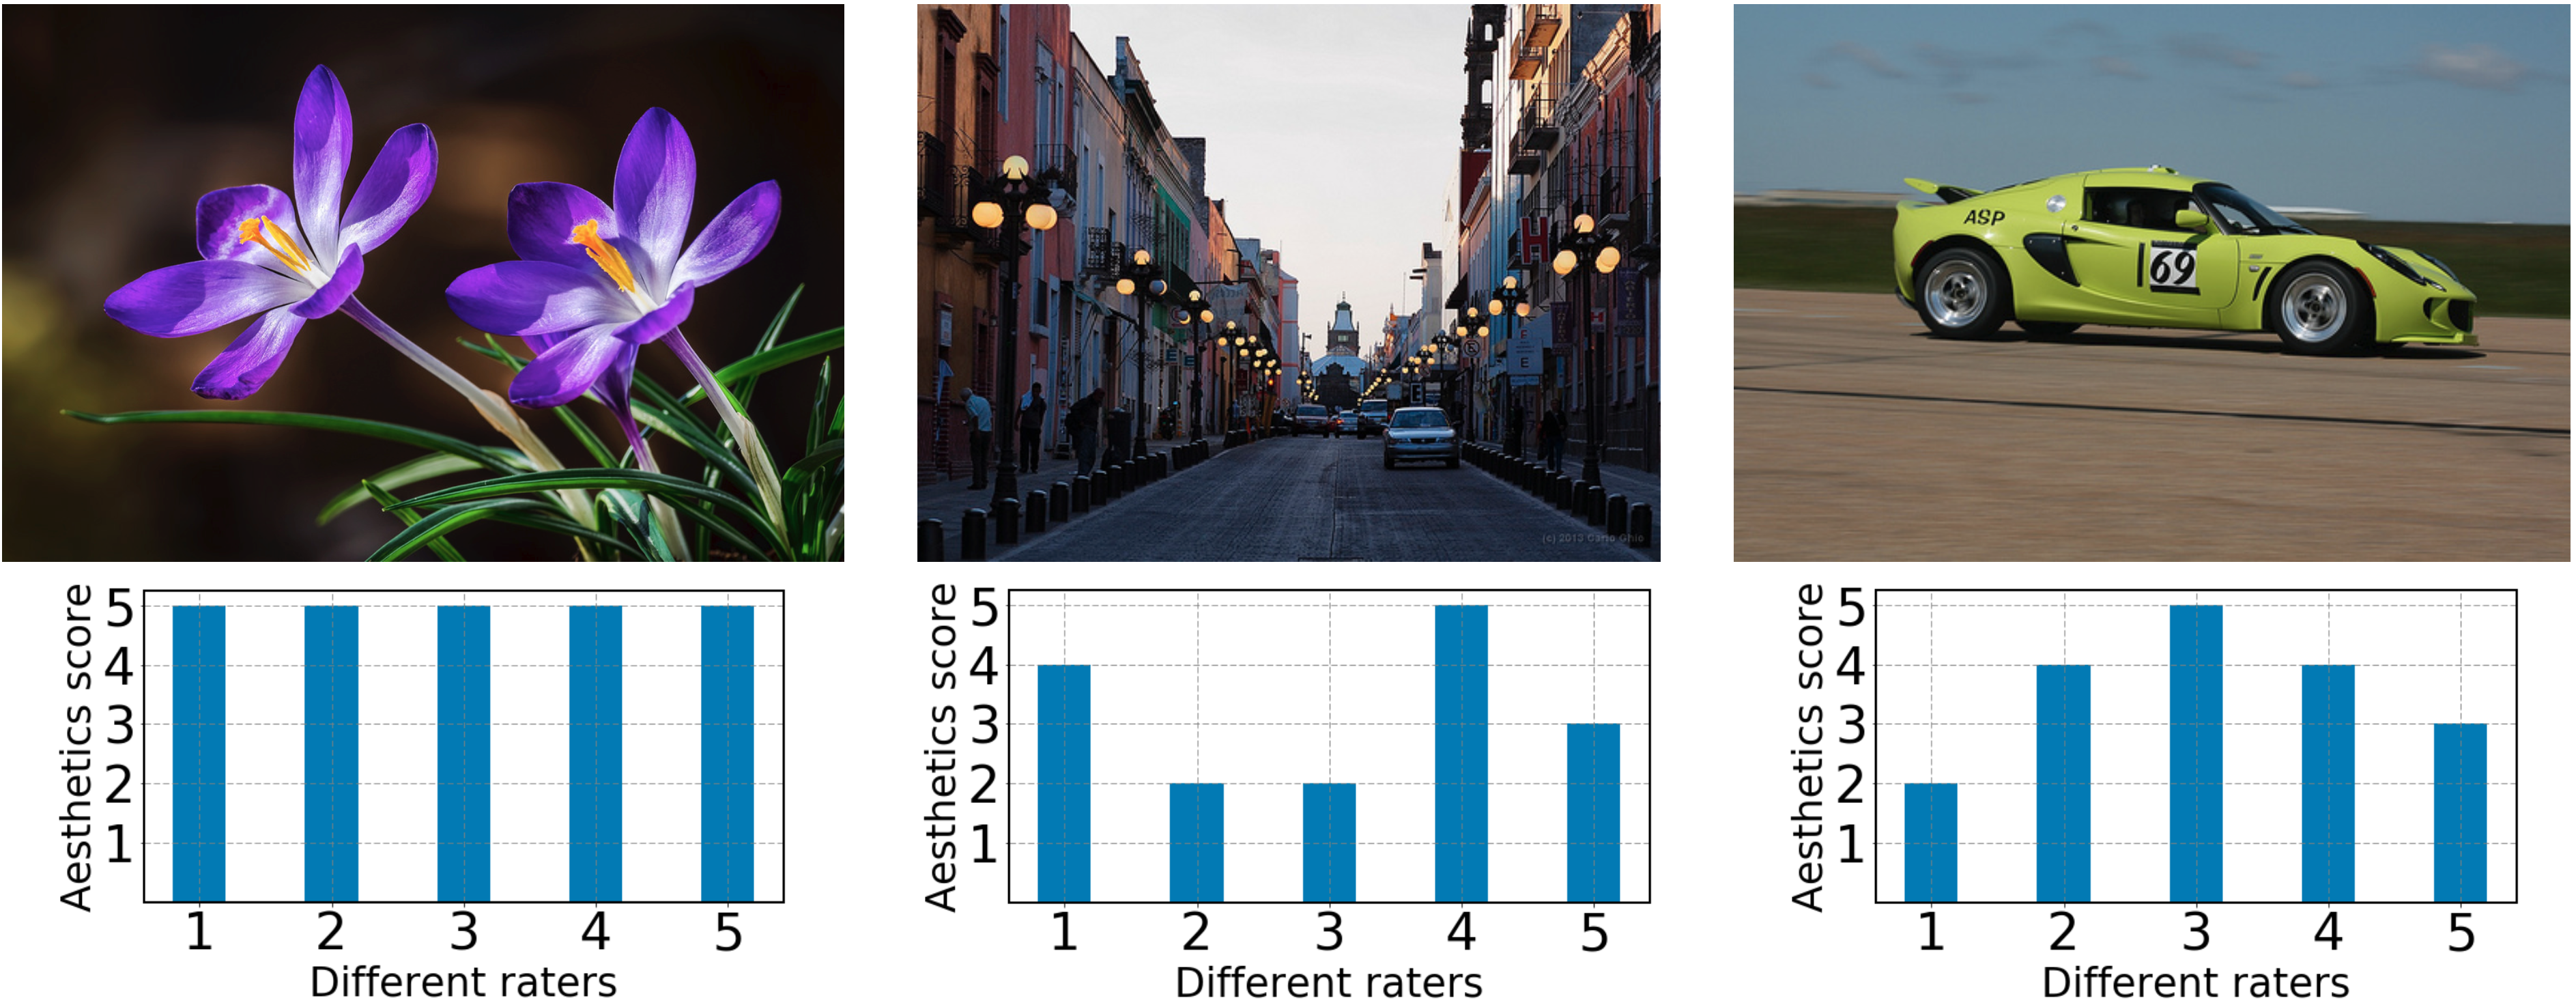
\includegraphics[width=1\columnwidth]{figures/demo1}
%\vspace{-0.3in}
\end{center}
\caption{Examples illustrating personal aesthetic preferences. Each image is rated by 5 different users. As can be seen, on the first example, ratings are consistent among the users while on the other two, different users manifest very different visual tastes. Individual users may have their unique preference with respect to visual attributes or contents of an image when they judge its aesthetic quality.} 
\label{demoImage}
\end{figure}
%****************************************************************

\section{Introduction}

Automatic assessment of image aesthetics is an important problem that has a variety of applications such as image search, creative recommendation, photo ranking and personal album curation, etc.~\cite{marchesotti2015discovering, lu2015deep}. It is a challenging task that requires high-level understanding of photographic attributes and semantics in an image. Only recently, there has been a significant progress due to the advancement in deep learning that can learn such high-level information effectively from data \cite{lu2014rapid, lu2015deep}. Although many successful deep learning-based approaches have been proposed for learning generic aesthetics classifiers, efforts on learning user-specific aesthetic models are quite limited. 

Image aesthetics rating is well known to be a highly subjective task as individual users have very different visual preferences. This has been observed in earlier rule-based photo ranking systems such as~\cite{yeh2010personalized, yeh2014personalized, vessel2014personalized}.  
For example, Figure~\ref{demoImage} shows example images and their aesthetic scores (1 to 5) rated by five different users following careful instructions. As can be seen, ratings for each image could vary significantly among the users. This is expected as different users may have very different opinions with respect to photographic attributes (composition, lighting, color) or semantic contents of the image (portrait, landscape, pets). Therefore, learning individual user's visual preference is a crucial next step in image aesthetics research.  

We refer to this problem as \textbf{personalized image aesthetics} and aim to address it by adapting a generic aesthetics model for individual user's preference. However, this is a challenging task as we typically need to learn such preference from a very limited set of annotated examples from each user. For example, in photo organization softwares, it is desired to minimize user's annotation effort. An effective strategy in such applications is to leverage active learning by automatically selecting representative images and suggest them to users for rating.

For investigating this problem with a learning-based approach, a labeled dataset with rater's identities are needed for training and evaluation purposes. Existing aesthetics datasets are not appropriate as they either do not have rater identities~\cite{murray2012ava} or are limited in size~\cite{kang2014convolutional}. Therefore, we introduce two new datasets specifically tailored for this task: (1) Flickr Images with Aesthetics Annotation Dataset (FLICKR-AES) which contains 40,000 Flickr images labeled by 210 unique Amazon Mechanical Turk (AMT)\footnote{https://www.mturk.com} annotators; (2) Real Album Curation Dataset (REAL-CUR) that contains 14 real user's photo albums with aesthetic scores provided by the album owners. 

To learn the average aesthetic preference of a typical user~\cite{bronstad2007beauty, kaplan1989experience}, we first use the relatively large FLICKR-AES dataset to train a powerful, generic aesthetics prediction model which performs competitively to the state of the art. Then, we present a novel approach for personalizing image aesthetics by adapting the generic model to individual users. To cope with a limited number of annotated examples from a user, we adopt a residual-based model adaptation scheme which is designed to learn a scalar offset to the generic aesthetic score for each user. 

Inspired by the studies~\cite{dhar2011high, luo2011content, murray2012ava} which leverage both aesthetic attributes and content information to improve the performance of generic aesthetics rating, we study feature representations effective for personalized aesthetics learning, and observed that features trained for generic aesthetics prediction, aesthetics attributes classification, and semantic content classification are all important for learning personalized image aesthetics models. We further show in experiments that our personalized aesthetics model with this combined feature representation significantly outperforms an existing collaborative filtering-based method.

Finally, we introduce an active personalized aesthetics learning algorithm for real-world application scenarios such as interactive photo album curation. Results demonstrate that our method compares favorably to typical active learning-based methods in the previous literature. 

Our main contributions are three-fold:
\begin{itemize}
\vspace{-0.1in}
  \item We address the problem of personalized image aesthetics, and introduce two new datasets to facilitate research in this direction.
  \vspace{-0.1in}
  \item We systematically analyze correlation between user ratings and image contents/attributes, and propose a novel approach for learning a personalized image aesthetics model with a residual-based model adaptation scheme.
  \vspace{-0.1in}
   \item We propose an active personalized image aesthetics learning algorithm for real-world image search and curation applications.
\end{itemize}


%****************************************************************
%****************related_work***********************************
\section{Related Work}
%\vspace{-0.1in}
\paragraph{Aesthetic quality estimation}

Earlier studies on image aesthetics prediction mainly focus on extracting hand-crafted visual features from images and mapping the features to annotated aesthetics labels by training classifiers or regressors~\cite{dhar2011high, ke2006design, luo2011content, marchesotti2011assessing}. 
%Early approaches adopt  generic image features such as SIFT \cite{lowe2004distinctive}, Fisher Vector \cite{perronnin2007fisher, perronnin2010improving} and bag of visual words \cite{su2011scenic} to predict aesthetics values. 
With the emergence of large-scale aesthetics analysis datasets such as AVA~\cite{murray2012ava}, a significant progress has been made on automatic aesthetics analysis by leveraging deep learning techniques~\cite{kang2014convolutional, lu2014rapid, lu2015deep, wang2016brain}. In~\cite{lu2014rapid, lu2015deep}, the authors show that using the patches from original images could consistently improve the accuracy for aesthetics classification. Mai \textsl{et al.}~\cite{mai2016composition} propose an end-to-end model with adaptive spatial pooling to process original images directly without any cropping. Kong \textsl{et al.}~\cite{kong2016photo} explore novel network architectures by incorporating aesthetic attributes and contents information of the images. However, all these works focus on learning generic aesthetics models.  
%\vspace{-0.3in}
\paragraph{Personalized prediction}
Collaborative filtering has been a popular algorithm for recommendation and learning personalized preferences. 
%For example, the online movie recommendation system of Netflix uses collaborative filtering to model customers' preferences based on their reviewing history and products' rating history \cite{koren2009matrix, shi2014collaborative, su2009survey}.  
Matrix factorization is a common approach that serves as the basis for most collaborate filtering methods~\cite{koren2009matrix, lee2001algorithms}. Matrix factorization-based methods are strictly limited to existing items already rated by some users and cannot be used to predict/recommend novel items for users. To overcome the limitations, several improvements have been introduced. For example, Rothe \textsl{et al.}~\cite{rothe2015some} introduce the visual regularization to matrix factorization that regresses a new image query to a latent space, while Donovan\textsl{et al.}~\cite{o2014collaborative} use a novel feature-based collaborative filtering that transforms the features of new item to latent vectors. Nevertheless, those approaches assume there are considerable overlaps among items rated by different users. In personalized image aesthetics, the sets of items rated by individual users may not necessarily be overlapping. For example, for photo curation, each user only rate their own personal images. Some earlier works on photo ranking~\cite{yeh2010personalized, yeh2014personalized} incorporate user feedback in the ranking algorithms but it is done by adjusting feature weights in an ad-hoc way instead of learning from data.  
%\vspace{-0.2in}
\paragraph{Active learning}
Active learning is an effective method to boost learning efficiency by selecting the most informative subset as training data from a pool of unlabeled samples. 
Samples with large uncertainties are likely to be chosen, whose ground-truth values are collected to update the models. 
However, most active learning methods deal with classification problems~\cite{tong2001support1, schohn2000less, settles2010active},  and in this study, our model aims to predict a continuous aesthetic score, which is formulated as a regression problem. Existing active classification approaches are not directly applicable to our problem because evaluation of uncertainties for unlabeled samples is nontrivial in regression methods such as support vector regression. Moreover, there is a risk of selecting non-informative samples which may increase the cost of labeling~\cite{willett2005faster, demir2014multiple}.  There have been a few attempts to apply active learning for regression problems, such as Burbidge \textsl{et al.}~\cite{burbidge2007active} which select unlabeled images with the maximal disagreement between multiple regressors generated from ensemble learning algorithms. Demir \textsl{et al.}~\cite{demir2014multiple} propose a multiple criteria active learning (MCAL) method that uses diversity of training samples and density of unlabeled samples. The active learning method introduced in our work differs from those works in that we define an objective function to select unlabeled images by considering the diversity and the informativeness of the images that are directly related to personalized aesthetics.
%\vspace{-0.1in}

%****************************************************************
%***************datasets*****************************************
%**************figure: two examples*********************************
\begin{figure*}
\centering
\subfloat[]{
  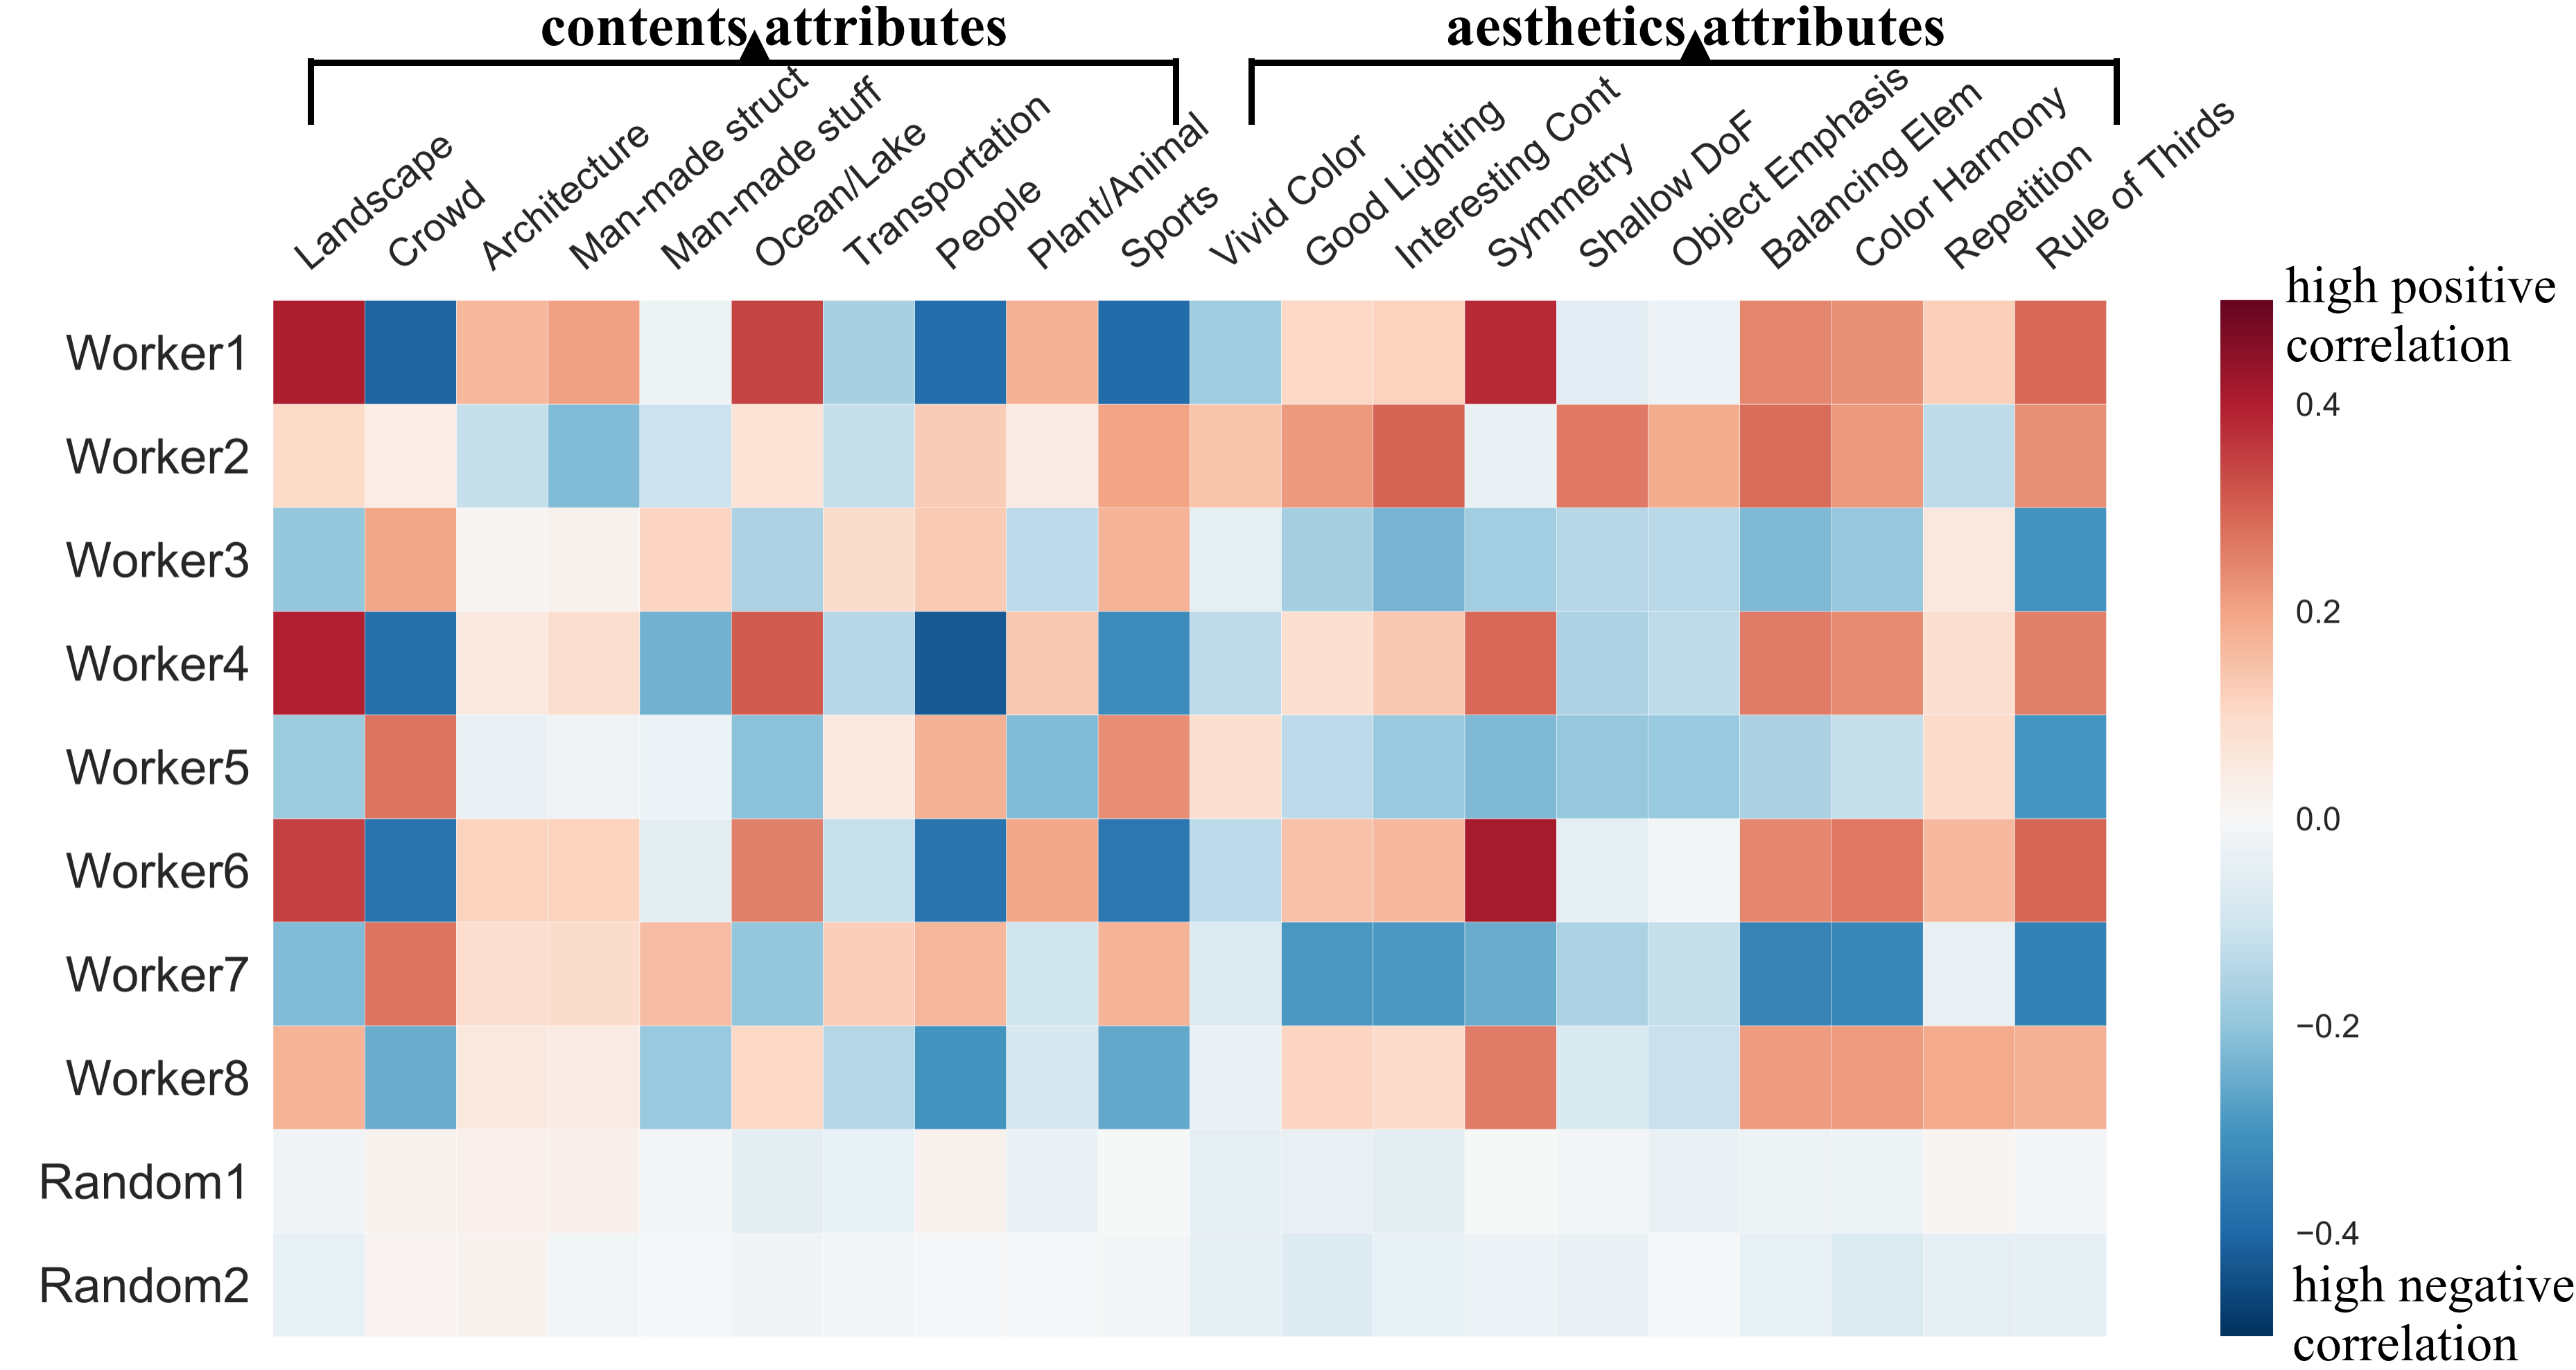
\includegraphics[width=1.7\columnwidth]{figures/amtRandomNew}\label{corrEx}
}\\
\vspace{-0.1in}
\subfloat[]{
  \includegraphics[width=1.8\columnwidth]{figures/turk1_4}\label{turker1_4}
}
\vspace{-0.15in}

\caption{(a) Ranking correlation between offsets and image attributes for randomly selected 8 AMT workers and 2 random users. (b) First row: Example images rated by Worker1. The user tends to assign higher scores to landscapes and lower scores to crowd scenes than the average ratings; Second row: Example images rated by Worker4. The user tends to assign lower scores to images containing symmetry attributes but higher scores to people scenes than the average ratings.}\label{corrTurker}
\vspace{-0.1in}
\end{figure*}
%****************************************************************
\section{Datasets}

%Existing aesthetics datasets either do not have rater identities\cite{murray2012ava} or have a limited number of annotated images\cite{kong2016photo}, thus are not suitable for the personalized aesthetics study. To overcome such limitations, we collected two new datasets and will later release them promote research investigation.
%\vspace{-0.15in}


\paragraph{FLICKR-AES} We download 40,000 photos with a creative commons license from Flickr\footnote{https://www.flickr.com} and collect their aesthetic ratings through AMT. The raw aesthetics scores range from 1 to 5 representing the lowest to the highest aesthetics level. Each image is rated by five different AMT workers and its ground truth aesthetics label is approximated to be the average of the five scores. In total, 210 AMT workers participated in the annotation of FLICKR-AES. 

We split the dataset into training and testing sets. Specifically, we select 4,737 images labeled by 37 AMT workers to include in the testing set. The number of photos each testing worker labeled ranges from 105 to 171 (avg. = 137). All the remaining 35,263 images annotated by the rest 173 workers are included in the training set. We leverage the latter for training both generic and personalized aesthetics models. With this split, we verified that the testing set does not have any images labeled by the workers in the training set, and vice versa. This allows us to simulate real application scenarios where each user only provide ratings on his or her own photos, and the algorithm cannot access those photos and ratings beforehand.

Compared to the existing aesthetics dataset with rater identities~\cite{kong2016photo}, FLICKR-AES is a much larger and more comprehensive dataset which has a more diverse and balanced coverage of contents. 

\paragraph{REAL-CUR}
In FLICKR-AES, aesthetics ratings are provided by AMT workers instead of actual owners of the photos in the dataset. For testing in the context of real-world personal photo ranking and curation applications, we collect another dataset composed of 14 personal albums (all from different people) and corresponding aesthetic ratings provided by the owners of the albums. The number of photos in each album ranges from 197 to 222 while the average is 205. As we only have one user rating for each photo, we instructed each user to go through their album multiple times to make the ratings consistent. To the best of our knowledge, this is the first aesthetics analysis dataset with real users' ratings on their own photos. We will make those datasets publicly available. More details and example images regarding the datasets are shown in the supplementary materials.



\section{Analysis of User Preferences}\label{analysis}
How significant are individual user's preferences relative to generic aesthetic perception? How are those preferences related to image attributes? In order to answer these questions, we perform the following correlation analysis between individual user's ratings and various image attributes using FLICKR-AES.

There are numerous image properties or attributes which could affect a user's aesthetics rating. Among them, we choose content attributes (semantic categories) and aesthetics attributes (e.g. rule-of-third, symmetry) as they are the most representative cues explored for aesthetics analysis and are proved effective for predicting aesthetic quality of an image\cite{dhar2011high, luo2011content}. We show  details on how to extract those attributes in Section~\ref{PAM}. 

We select 111 AMT workers from the training set who have labeled at least 172 images (avg. = 1,550), and treat them as individual users. For each user, to measure the correlation of the preference and the content/aesthetics attributes, we use Spearman's rank correlation ($\rho$) \cite{myers2010research} which is calculated as $\rho = 1 - 6\frac{\sum_{i=1}^{N}{(r_i - r_{i}^{'})}^2}{N^3 - N}$, where $r_i$ is the rank of the $i$-th item when sorting the scores given by the first metric in descending order and $r_{i}^{'}$ is the rank for the scores given by the second metric. $\rho$ ranges from -1 to 1 and a higher absolute value indicates stronger correlation between the first metric and the second metric. 

Directly measuring the correlation between user's absolute aesthetics scores and image attributes cannot properly reflect user's preference, as the correlation values in this case are dominated by the average ratings of each image. Therefore, we compute the offset (or residual) of a user's score to the ground truth (average) score, and measure correlation between offset values and image attributes instead. We randomly select 8 AMT workers and show the results in Figure~\ref{corrEx}, in which dark red color indicates a user prefers these attributes, while dark blur color means the user has relatively lower scores on images with those attributes. It clearly shows that the deviation of each user's ratings (w.r.t. image attributes) are unique. We further visualize example images rated by Worker1 and Worker4 in Figure~\ref{turker1_4}. As we can see, Worker1 prefers landscape images versus images of crowds while Worker4 prefers images with symmetry attributes over images of people. 

To understand the significance of the correlation versus randomness of users' labels, we additionally create two ``random '' users as the baseline. The two random users are generated by randomly sampling 1,000 images from the training set as their annotated images. The score for each image is set to the ground-truth score (i.e. the average rating of five AMT workers) perturbed by a zero-mean Gaussian random noise with standard deviation of 0.2 and 2, respectively. We choose those standard deviations to simulate two ``average'' users with a relatively small and a relatively large amount of label offsets deviated from the generic scores.
The correlations of their offsets with attributes are also included in Figure~\ref{corrEx}, which show no statistically meaningful preference as expected. Compared with ``random'' users, the correlations on actual users are much stronger, demonstrating that their preferences are indeed related to content and aesthetics attributes instead of random deviations.

For each user, we also compute the sum of the absolute values of the correlation and compare the value with two random users. We run the experiments for 50 times and report the average for the two ``random'' users. We find all the 111 actual users have higher average correlation scores than the ``random'' users, showing that the correlations are statistically meaningful. 

The analysis demonstrates that score offsets are very effective cues revealing user preferences regarding aesthetics on content and aesthetics attributes. Motivated by this, we derive a novel residual (offset)-based model for learning personalized aesthetics in the next section. 
%We calculate the ranking corrleation between the with the 


%****************************************************************
%*************************************approach****************************************
%*************figure: offset pipeline and attributes network*************
\begin{figure}
\centering
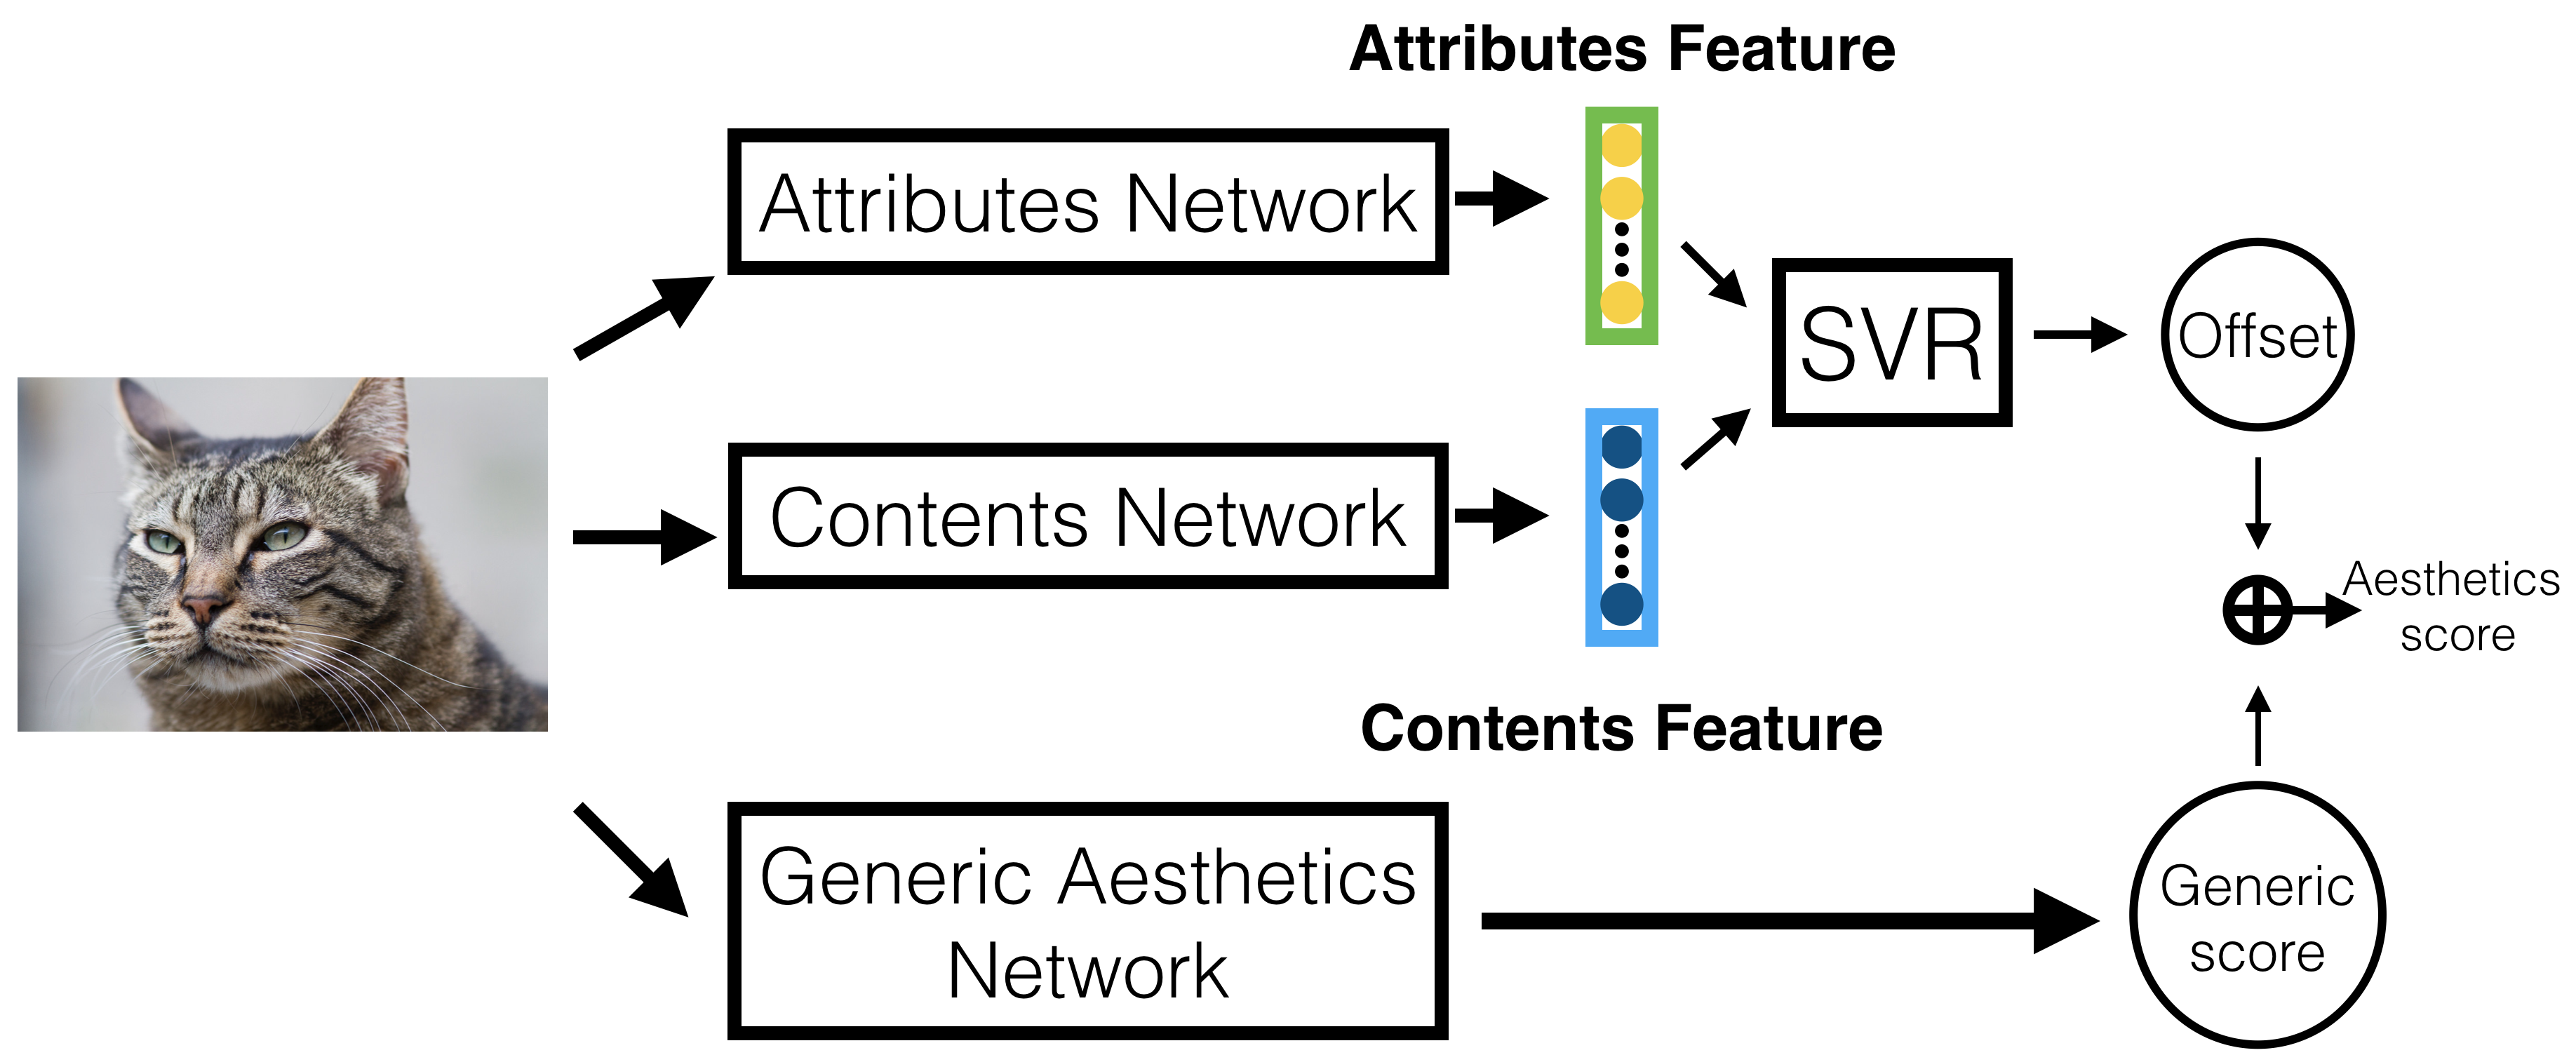
\includegraphics[width=1.0\columnwidth]{figures/offset} 
\caption{An overview of the proposed residual-based personalized aesthetics model.}
\label{offset_a}
\end{figure}
%****************************************************************


%*****************approach****************************************
\section{Approach}
In this section, we first introduce our proposed approach to learn personalized aesthetics models by adapting a generic aesthetics model to individual users and then continue to derive an active learning algorithm for real-world photo curation applications. 
\subsection{Personalized aesthetics model (PAM)}\label{PAM}

In real-world photo ranking and curation applications, users often provide a very limited number of aesthetic ratings or feedbacks to their own photos. The lack of labeled exampled makes it difficult to train a meaningful personalized aesthetics model from scratch. Traditional recommendation-based approaches such as collaborate filtering may not be very effective as they require significant overlapping of items rated by different users. In photo curation applications, the user-item matrix could be too sparse to learn effective latent vectors\cite{o2014collaborative}. 

In order to learn an effective personalized model with good generalization, we aim to capture not only the common aesthetic preference shared across individuals\cite{bronstad2007beauty} but also the unique aesthetic preference by each individual \cite{yeh2014personalized, vessel2014personalized} .
%, which are two vital importance components to understand personalized image aesthetics. 
Following this idea, we propose to leverage the generic aesthetics model trained to predict the average user's ratings, and focus personalized aesthetics learning on modeling the deviation (residual) of individual aesthetics scores from the generic aesthetics scores. We first train a generic aesthetics model using the FLICKR-AES training set by treating the average rating as the ground truth aesthetic score. Then, given an example set rated by each user, we apply the generic model to each image in the set to compute the residual scores between the user's ratings and the generic scores. Finally, we train a regression model\cite{chang2002training} to predict the residual scores. The overview of the approach is illustrated in Figure~\ref{offset_a}.

%The overview of the approach is illustrated in Figure~\ref{offset_a}. The details of the generic aesthetics model as well as the SVR personalization model will be described in details respectively.

\paragraph{Generic aesthetics prediction}
Recent studies\cite{kong2016photo, lu2014rapid, lu2015deep} have achieved promising results on generic image aesthetics prediction using deep learning. Inspired by these works, we train a deep neural network to predict genetic aesthetic scores. It has the same architecture as in~\cite{ioffe2015batch} except that we trimmed the number of neurons in the second-to-the-last layer, which we found makes the training more efficient and yields better accuracies. We tested different combinations of loss functions as in~\cite{kong2016photo}, but experimentally found that the Euclidean loss function alone works the best on our dataset. We also verified that our generic model achieves results comparable to the recent state of the art by Kong et al.~\cite{kong2016photo} on their AADB dataset~\cite{kong2016photo}.
%The details of the last inception are illustrated in Table~\ref{inception}.  Besides the trimmed inception, a dropout layer with 50\% ratio is added after the last pooling layer. 
%In order to predict continuous aesthetics values, we use Euclidean loss to train the network. 
%\vspace{-0.1in}
%\begin{equation}
%\small
%loss_{aes} = \frac{1}{2N} \sum_{i=1}^{N} {\left \| y_{i}^{'} - y_i \right %\|_{2}^{2}}
%\vspace{-0.1in}
%\end{equation}
%where $y_i$ is the ground truth rating from AMT for the $i-th$ image, and %$y_{i}^{'}$ is the corresponding predicted aesthetics score. 
%Only one loss function is used at the end because we tried the multiple loss functions as in \cite{ioffe2015batch} but found the L2 loss-alone works the best for the FLICKR-AES dataset.

\paragraph{Residual learning for personalized aesthetics}
With the generic aesthetic scores, we can compute residual scores (offsets) for the example images by subtracting them from ratings by each user. Our goal is then reduced to learn a regressor to predict the residual score given any new image.

Due to the lack of annotated examples from each user, training such regressor directly from an image is not practical. Therefore, we propose to use high-level image attributes related to image aesthetics to form a compact feature representation for residual learning.
We consider both aesthetic and content attributes inspired by previous studies\cite{kong2016photo, dhar2011high, lu2014rapid, marchesotti2015discovering, luo2011content, murray2012ava} for automatic assessment of generic aesthetics.   
%For example, some user may prefer portrait photos over landscape photos, and different users may have different tastes on colorful images. 

Given the features, we simply use the support vector regressor with a radial basis function kernel to predict the residual score as shown in Equation~\ref{svr},
%**************************SVRegression************************
\begin{equation}
\begin{split}
& {min} \hspace{0.3cm}\frac{1}{2} \textbf{w}^T \textbf{w}+C(\nu\epsilon  + \frac{1}{l}\sum_{i=1}^{l}(\xi_{i}+\xi_{i}^{*} ) )\\
& s.t. \hspace{0.4cm}  (\textbf{w}^T\phi(\textbf{x}_i) + b) - y_i\leq \epsilon  + \xi _{i},\\
& \hspace{0.9cm}   y_i - (\textbf{w}^T\phi(\textbf{x}_i) + b) \leq \epsilon  + \xi _{i}^{*},\\
&\hspace{0.9cm}   \xi_{i},\xi _{i}^{*}\geq 0, i=1,...l,  \epsilon \geq 0.
\end{split}
\label{svr}
\end{equation}
\vspace{-0.1in}

%****************************************************************
where $\textbf{x}_i$ is the concatenation of aesthetic attribute features and content features, $y_i$ is the target offset value, $C$ is the regularization parameter, and $\nu$ ($0 < \nu \leq 1$) controls the proportion of the number of support vectors with respect to the number of total training images. We discuss the details of the feature vector $\textbf{x}_i$ in the following.

%The preferences of users usually lie on certain image content or image style.

\paragraph{Feature representation for personalized aesthetics}
We first leverage the existing AADB\cite{kong2016photo} dataset which contains around 10,000 images labeled with ten aesthetic attributes\footnote{The aesthetics attributes include \textsl{interesting content (IC)}, \textsl{object emphasis (OE)}, \textsl{good lighting (GL)}, \textsl{color harmony (CH)}, \textsl{vivid color (VC)}, \textsl{shallow depth of field (DoF)}, \textsl{rule of thirds (RoT)}, \textsl{balancing element (BE)}, \textsl{repetition (RE)} and \textsl{symmetry (SY)} } to train our aesthetic attribute features. Due to the limited number of training images provided by AADB, we use our trained generic aesthetics network as a pre-trained model, and fine-tune it by multi-task training, i.e. attribute prediction using AADB and aesthetics prediction uisng Flickr-AES. We use the Euclidean loss for both attribute prediction and aesthetics prediction, and fix all the earlier layers of the generic model and only fine-tune its last shared inception layer and the prediction layers. Given the fine-tuned network, we use the $10$-dimensional responses as the aesthetic attributes feature vector $f_{attr}$. Experiments show that the attributes prediction performance of our jointly trained network is significantly better than the one from\cite{kong2016photo}, as shown in Table~\ref{attributes}. It demonstrates that features learned from larger-scale aesthetics dataset could also benefit attributes prediction attribute annotations.

As for the content features, we use the off-the-shelf image classification network\cite{ioffe2015batch} to extract semantic features (avg pool) from each image. In order to generate compact content attribute features, we first use $k$-means to cluster the images from the FLICKR-AES training set into $k=10$ semantic categories using the second-to-the-last inception layer output as the feature. We then add a $k$-way soft-max layer on top of the network and fine-tune the layer with the cross-entropy loss. The $10$-dimensional outputs of the network are defined as the content attributes feature vector $f_{cont}$. We concatenate the two feature vectors $\textbf{x} = [f_{attr}, f_{cont}]^T$, to form our final feature representation to personalized aesthetics learning. Experiments show the concatenation of attributes and content features achieve better results than using each of them alone.
%***********************greedy algorithm******************************************
\begin{algorithm}
\small
    \SetKwInOut{Input}{Input}
   \Input{Unrated photo set  $\mathcal{N}=\{{p_i }\}_{i=1,K}$, the aesthetic feature vectors $v_i$, the maximum number of example ratings $m$;}
    Initialize the set of rated examples as: $\mathcal{R} = \emptyset $ \;
    Randomly select a subset $\mathcal{S}$ of $\floor{K/10}$ images from $\mathcal{N}$ and move them to $\mathcal{R}$: $\mathcal{N} = \mathcal{N} \setminus \mathcal{S}$, $\mathcal{R} = \mathcal{R} \cup  S$ \;

    \While{$|\mathcal{R}|< m$}{
   Train a regressor to predict the residual score $ \{r_i \} $\;
   Calculate the weight for each annotated image   
   \begin{equation}
   %\begin{split}
   %&
    w_i =(1 - \frac{\left | r_i \right |}{\sum_{i=1}^{|\mathcal{R}|}(\left | r_i \right |)}) , p_i \in \mathcal{R}
   %\end{split}
   \label{weight}
    \vspace{-0.2in}
   \end{equation}  \
   
    Find $p_q$  that
    \begin{equation}
    %\centering
    %\begin{split}
 \underset{q}{max} \hspace{0.1cm} \sum_{j=1}^{|\mathcal{R}|}w_j dist(v_q, v_j),    p_q \in \mathcal{N},  p_j \in \mathcal{R}\;
    %\end{split}
    \label{objective}
     \vspace{-0.15in}
    \end{equation}
    \noindent

    Add the selected image to $R$ and update $N$:
    $\mathcal{R} = \mathcal{R} \cup  \{p_q \} $ and $\mathcal{N}\setminus p_q$ \;
    %Remove $p_q$ from $N  $\;
    }
    \caption{Active-PAM}
\label{alg}
\end{algorithm}
\vspace{-0.05in}

%***************************************************************

%\subsection{personalize aesthetics model}
\subsection{Active personalized image aesthetics learning (Active-PAM)}\label{Active}
%why we need select training images then how to do this 
%active learning for personalize aesthetics
In real-world applications such as interactive photo curation, users can continuously provide ratings regarding their aesthetics preference during the photo selection and ranking process\cite{yeh2010personalized, yeh2014personalized}. Instead of waiting for users to provide ratings on arbitrary images, we can use active learning to automatically select the most representative images for users to rate, and learn from their feedback online. To minimize the user effort, we propose a new active learning algorithm to optimize sequential selection of training images for personalized aesthetics learning. Specifically, we consider the following two criteria: 1) the selected images should cover diverse aesthetic styles as quickly as possible with minimum redundancy; 2) the images with large residual scores between user's ratings and the generic aesthetics scores are more informative. 

Based on these criteria, we design our active selection algorithm as follows. For each image $p_i$ in the collection $\mathcal{N}$, we denote its aesthetics score predicted by the generic aesthetics network as $s_i$, features extracted at the second-to-the-last layer output as $f_i$. The aesthetic feature capturing the aesthetic styles of the image can then be represented as $v_i = [w_{a}f_i, s_i]$, where $w_a$ is a constant balancing the two terms. We can then measure the distance between any two images $p_i$ and $p_j$ using the Euclidean distance $dist(v_i, v_j)$.

Given a set of images $\mathcal{R}$ already annotated by the user, for each remaining image $p_i$ in the album, we can calculate the sum of distances between $p_i$ and any image $p_j$ in $\mathcal{R}$, $ d_i = \sum_{j=1}^{|\mathcal{R}|} dist(v_i, v_j)$, $p_j\in \mathcal{R}$. At each step, we can choose the image with the largest $d_i$ according to the first criterion. In order to incorporate the second criterion at the same time, we can encourage selecting the image producing large residuals in $\mathcal{R}$. We denote the residual score as $r_j$ and assign weight $w_j$ to each image using Equation~\ref{weight}. We apply the weights to the overall distance, resulting in Equation~\ref{objective}. The details of the active learning algorithm are described in Algorithm~\ref{alg}.




%*******************************attributes table********************
\begin{table}
\begin{center}
\small
\centerline{
\begin{tabular}{C{1.7cm} C{0.9cm} C{0.9cm} C{0.9cm} C{0.9cm} C{0.9cm}} 
\Xhline{2.5\arrayrulewidth}
 &VC&GL&IC&SY&DoF \\% [0.5ex] % inserts table
\hline % inserts single horizontal line
Baseline & 0.5759 & 0.3770 & 0.4854 & 0.2283 & 0.5071 \\ %[1ex] 
Our Results & \textbf{0.6938} & \textbf{0.4963} & \textbf{0.5641} & \textbf{0.2558} & \textbf{0.5476} \\% [1ex] adds vertical space
%hline %inserts single line
\Xhline{1.5\arrayrulewidth}
& OE&BE&CH&RE&RoT\\ %[0.5ex] % inserts table
\hline
Baseline & 0.5728 & 0.2035 & 0.4808 & 0.3150 & 0.2174\\%[1ex]
Our Results & \textbf{0.6718} & \textbf{0.3104} & \textbf{0.5176} & \textbf{0.3749} & \textbf{0.2737} \\% [1ex] adds vertical space
\Xhline{2.5\arrayrulewidth}
\end{tabular}
}
\end{center}
\vspace{-0.1in}
\caption{Attributes comparison of the baseline\cite{kong2016photo} and our results. Both calculated by correlation $\rho$.  Jointly training attributes and aesthetics improves the attributes prediction.} % title of Table
\label{attributes} % is used to refer this table in the text
\end{table}
%******************************************************************************

%******************************************************************************
%******************experiments*************************************************
%*************show 2 examples*********************************
\begin{figure}
\centering
\subfloat[One example user from FLICKR-AES]{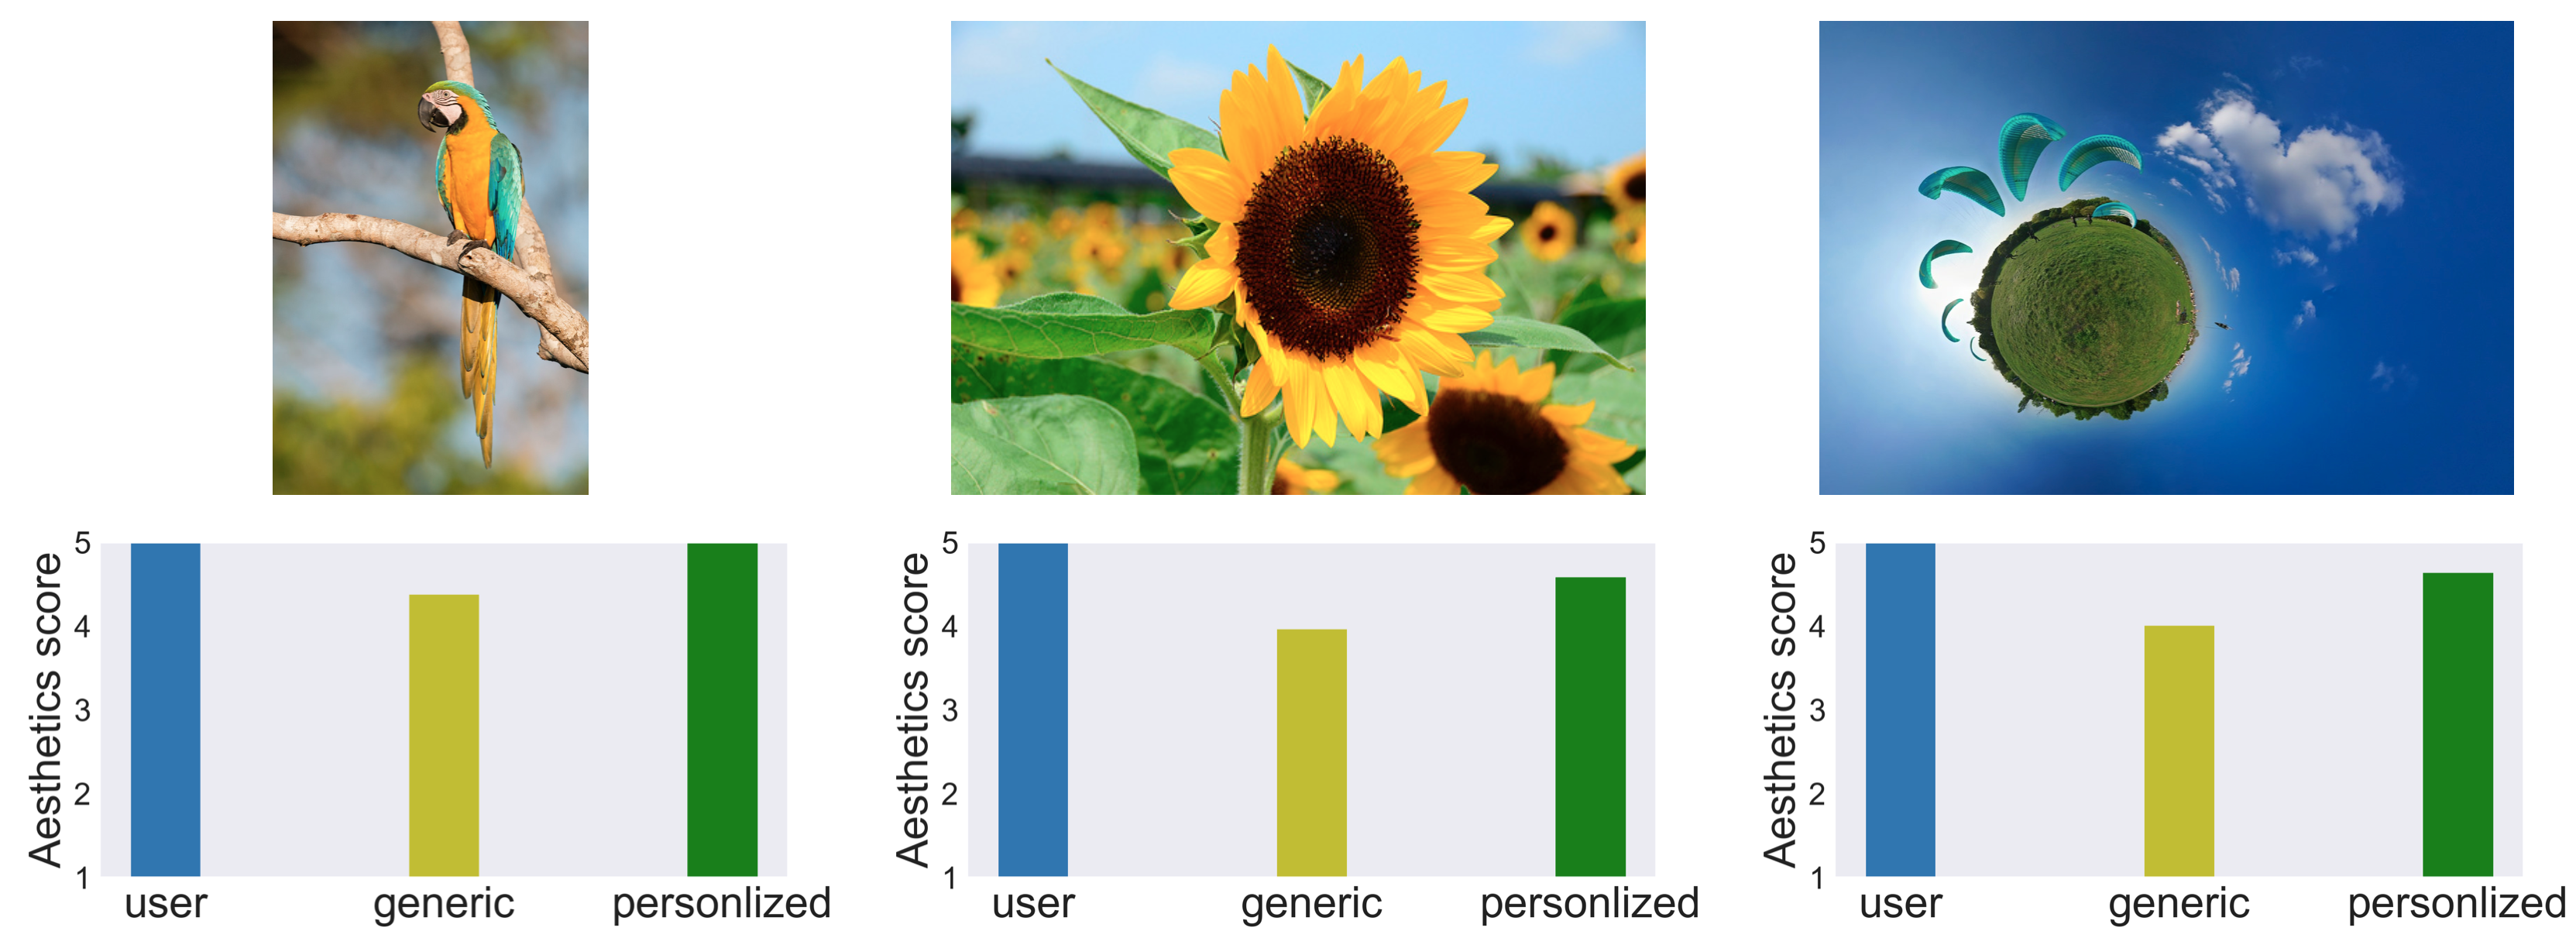
\includegraphics[width=1\columnwidth]{figures/user1_new}}%3.5in
\\
\subfloat[One example user from REAL-CUR]{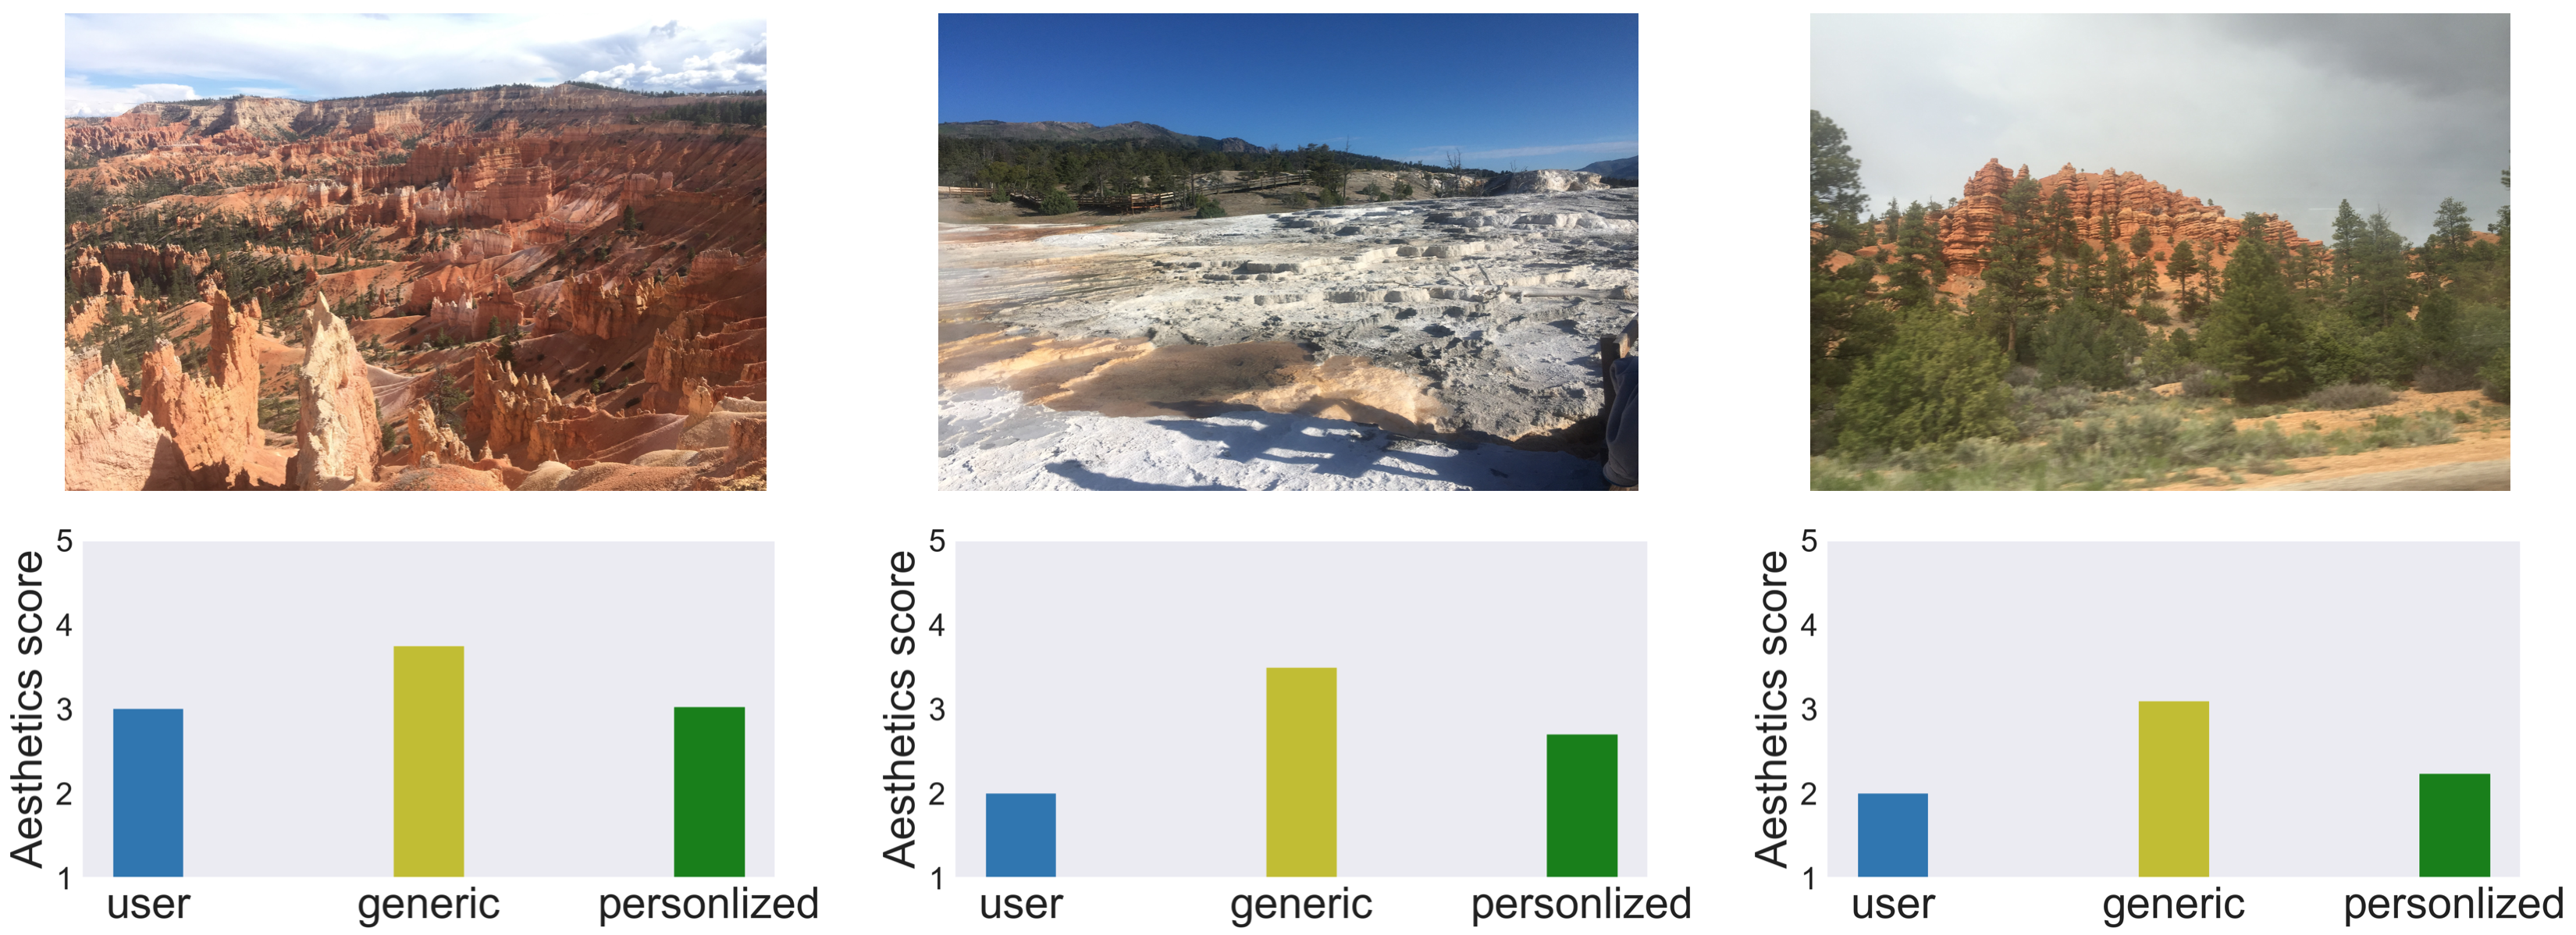
\includegraphics[width=1\columnwidth]{figures/user2_new}}
\caption{Example results of personalized aesthetics prediction from two users. The examples in (a) comes from FLICKR-AES and the examples in (b) comes from REAL-CUR. The blue bar is the user rating, the yellow bar is the generic aesthetics prediction and the green bar is the personalized aesthetics prediction for this user. As can be seen, our personalized model more accurately predicts user ratings than the generic model.
}
\vspace{-0.2in}
\label{examples}
\end{figure}

%******************************************************************************
%****************************************************************
\section{Experiments}

In this section, we present the experimental evaluation of our personalized aesthetics model (PAM) and our active learning approach (Active-PAM) on both the FLICKR-AES and the REAL-CUR datasets.
Figure~\ref{examples} introduces visual examples to show how the model works. 
\subsection{Implementation details}
%\paragraph{Implementation}
 The earlier layers of our generic aesthetics network are initialized from the Inception-BN network \cite{ioffe2015batch}, whereas the last trimmed inception module is randomly initialized using ``Xavier''. The network is then fine-tuned on FLICKR-AES. During training, images are warped to $256 \times 256$ and then randomly cropped to $224 \times 224$ before feeding into the network. The learning rate is initialized as 0.001 and periodically annealed by 0.96. The weight decay is 0.0002 and the momentum is 0.9. 


%\paragraph{Evaluation results}
%The evaluation of generic model is measured by the Spearman's rank correlation ($\rho$) \cite{myers2010research} between predicted aesthetics scores and the ground-truth values. The correlation is calculated as $\rho = 1 - 6\frac{\sum_{i=1}^{N}{(r_i - r_{i}^{'})}^2}{N^3 - N}$, where $r_i$ is the rank of the $i$-th item when sorting the ground truth scores from high to low and $r_{i}^{'}$ is the rank for the estimated score. $\rho$ ranges from -1 to 1 and higher value indicates better correlation between the predicted scores and the ground-truth scores. The correlation for the aesthetics generic model is 0.702. Table~\ref{attributes} shows the correlation on ten attributes. Interestingly, we found that the prediction of the attributes is significantly better than the one from\cite{kong2016photo}, benefiting from larger training dataset in generic model.

\subsection{Evaluation on personalized aesthetics models}

To evaluate our personalized aesthetics model (PAM), we compare PAM with a baseline model as well as a commonly used collaborate filtering approach and show that PAM works significantly better than the other two. We further analyze the effectiveness of content and aesthetic attribute features used in our model.


\paragraph{Comparison with other methods.} We compare PAM with two other methods: 1) a baseline SVM regressor that directly predicts user-specific aesthetics scores on test images based on user-provided training images, and 2) a commonly used collaborate filtering approach, non-linear Feature-based Matrix Factorization (FPMF), which achieves better performance than other matrix factorization approaches on individual color aesthetics recommendation\cite{o2014collaborative}. In both methods, we use the same content and aesthetic attribute features as in our method. 



%The non-linear FPMF trains a one layer neural network to map the image features from training set into latent space, therefore it can predict user's preference on the images that are not contained in the training set\cite{o2014collaborative}. The one layer neural network in non-linear FPMF includes 200 logistic units that can be trained by back-propagation and the dimensionality for the latent space is 15. 

We evaluate these three methods on the test workers in FLICKR-AES. During evaluation, for each test worker, we randomly sample $k$ images from the ones he or she labeled, and use them as training images. All the remaining images are then used for testing. For the non-linear FPMF, all the other workers in the FLICKR-AES training set are also included for training. Due to the randomness of training image selection, we run the experiments 50 times for each test worker, and report the averaged results as well as the standard deviation. 

Following \cite{kong2016photo}, ranking correlations are used to measure the consistency between the predictions and the ground-truth user scores. The mean ranking correlation of the generic aesthetics model over all the test workers are 0.514. In Table~\ref{mfNfeature}, we show the improvement in terms of correlation for each method compared with the generic model, with $k = 10$ and $k = 100$, respectively. We can see the SVM model that directly predict scores does not work on this problem, as its results are even worse than the ones from the generic model. It tries to directly learn each user's flavor regarding aesthetics from very limited data without considering generic aesthetics understanding, which is accordingly very unstable and hardly generalizable. By contrast, our method (last row in Table~\ref{mfNfeature}) works even with 10 training images, and has much more significant improvement with more training examples. It validates the design of our residual-based model, which fully leverages the common understanding of aesthetics existing in the generic aesthetics network, and focuses on the score offsets that directly correspond to users' unique preference compared with generic aesthetics. Our model also significantly outperforms FPMF, which only has marginal improvement even when using 100 training images.

\paragraph{Ablation study on features.}  We also show the results of PAM when trained only using the content feature or only using the aesthetics attribute feature, respectively, in the 3rd and 4th row in Table~\ref{mfNfeature}. We can see that both content and aesthetics attributes can be used to model personalized aesthetics, as the correlations with users' ground truth scores also increase  when using more user provided training images. Nevertheless, using both features gives the best performance. It further demonstrates that users' preference on image aesthetics are related to both image content and aesthetic attributes.


\subsection{Evaluation on active learning}

%\paragraph{Visual vector for training set selection}As described in Section~\ref{Active}, we use the aesthetic features to calculate the aesthetic dissimilarity between images and select images for active learning instead of using other features to encode image content and style information, (e.g, the content feature and attributes feature used to learn the personalized aesthetics model). We show the results using different features in active learning as in  Figure~\ref{5b}. The comparison demonstrates using generic aesthetics score and aesthetics features to select training samples is better than using attributes and contents features, as aesthetics features could better capture the diversity of images. We also show the results of using different criteria for the Active-PAM in Figure~\ref{5b}, which demonstrate using two criteria  (diversity and informativeness) is better than just considering one criteria.



\paragraph{Comparison with other methods.} We compare our method with three other active learning methods: 1) Greedy\cite{yu2010passive}, which selects the sample that has the minimum largest distance to the already selected samples at every iteration;  2) MCAL\cite{demir2014multiple}, which chooses samples by clustering the candidate images to be selected and selected images that are not support vectors;  3) Query by Committee (QBC) \cite{burbidge2007active}, which generates a committee of models by using ensemble algorithms. In our experiment, we generate 5 committees using Bagging for QBC \cite{mamitsuka1998query}. We choose these three methods for comparison because they deal with regression problem, whereas classic active learning approaches\cite{tong2001support1, demir2014multiple} for classification are not applicable here, as their criteria such as margin-based sampling are not suitable for continuous aesthetics scores. In addition, we also add another baseline where all the images are randomly selected.

To evaluate an active learning method, we start with 10 randomly selected images to train the initial PAM. Based on the initial results, we keep selecting new images from user's photo album using the active learning methods and updating the PAM model, until the number of selected images reaches 100. Different methods may select different images for model update. To compare these methods on the same test images, we chose to use the entire photo album for evaluation. It is also consistent with the real application scenario of personalized aesthetics, where the algorithm is able to access and actively select any image in the photo album, and the quality of overall ranking on all images in the album is the most important factor for the user.

Due to the randomness in the initialization of the PAM model, we repeat the experiments 10 times for each method, and measure the average performance. The results are shown in Figure~\ref{fig:testresults}. Our active selection method outperforms all the other baseline methods as well as random selection.

To further examine the generalizablility of the PAM models updated by different active learning approaches, instead of evaluating on the entire photo album, we remove all the images that have already been selected for model update, and only evaluate on the remaining images the model has not seen before.  We note that it is not a totally fair comparison, as images used for evaluation may be different for different active learning approaches, due to the different images they selected for model update. But it still gives us a sense how the model works on new images. The results are reported in Figure~\ref{fig:testresults2}. When evaluating on those unseen images, the PAM model updated by our active selection performs significantly better.
%\vspace{-0.1in}
%\subsection{Generalization study}
%\vspace{-0.1in}
%Moreover, the Active-PAM can be applied to any generic aesthetic model to accommodate user preference. To validate the generalizability of Active-PAM, we use the network from \cite{kong2016photo} as the generic aesthetics model instead of our own trained network, and test the results of personalized image aesthetics. The reason for using the model developed in \cite{kong2016photo} instead of other generic models is that the model is trained on the dataset (AADB) that collected from natural images and with rater identity. So we can run the experiment on the same dataset by splitting images according to rater identity. We use 28 workers in AADB who label 100 to 200 images to test the performance. The result is shown in Figure~\ref{shuModel_fig}, which indicates Active-PAM can be applied to different generic models for learning individual user's aesthetics model. The improvement is less significant than the one using our trained generic aesthetics network. It indicates that a  better generic aesthetics model could help improve personalized image aesthetics more.




%******************************************************************************

%**********************Table: Feature & MF********************
\begin{table}
\begin{center}
\small
\centerline{
\begin{tabular}{|C{3.55cm}| C{1.93cm}| C{1.93cm} |} 
\hline
 &  10 images &  100 images\\ \hline
Direct score prediction  &-0.352 $\pm$ 0.050  & -0.176 $\pm$ 0.064 \\
non-linear FPMF\cite{o2014collaborative} & -0.001 $\pm$ 0.003 & 0.010 $\pm$ 0.007\\ \hline
PAM (only attribute) & 0.004 $\pm$ 0.003& 0.025 $\pm$ 0.013\\
PAM (only content)& 0.001 $\pm$ 0.004  &0.021 $\pm$ 0.017\\
PAM (content and attribute) &\textbf{0.006 $\pm$ 0.003} &\textbf{0.039 $\pm$ 0.012} \\
\hline
\end{tabular}
}
\end{center}
\vspace{-0.1in}
\caption{Comparison with direct score prediction (using SVM), non-linear FPMF\cite{o2014collaborative}, PAM with only content feature, PAM with only attribute feature and PAM with both features using different number of training images from each worker. The results are average correlation improvement.} % title of Table
%\vspace{-0.15in}
\label{mfNfeature} % is used to refer this table in the text
\end{table}
%*****************************************************************************


%**************Different Dataset2*********************************
\begin{figure}
\begin{center}
\subfloat[Results on FLICKR-AES]{
  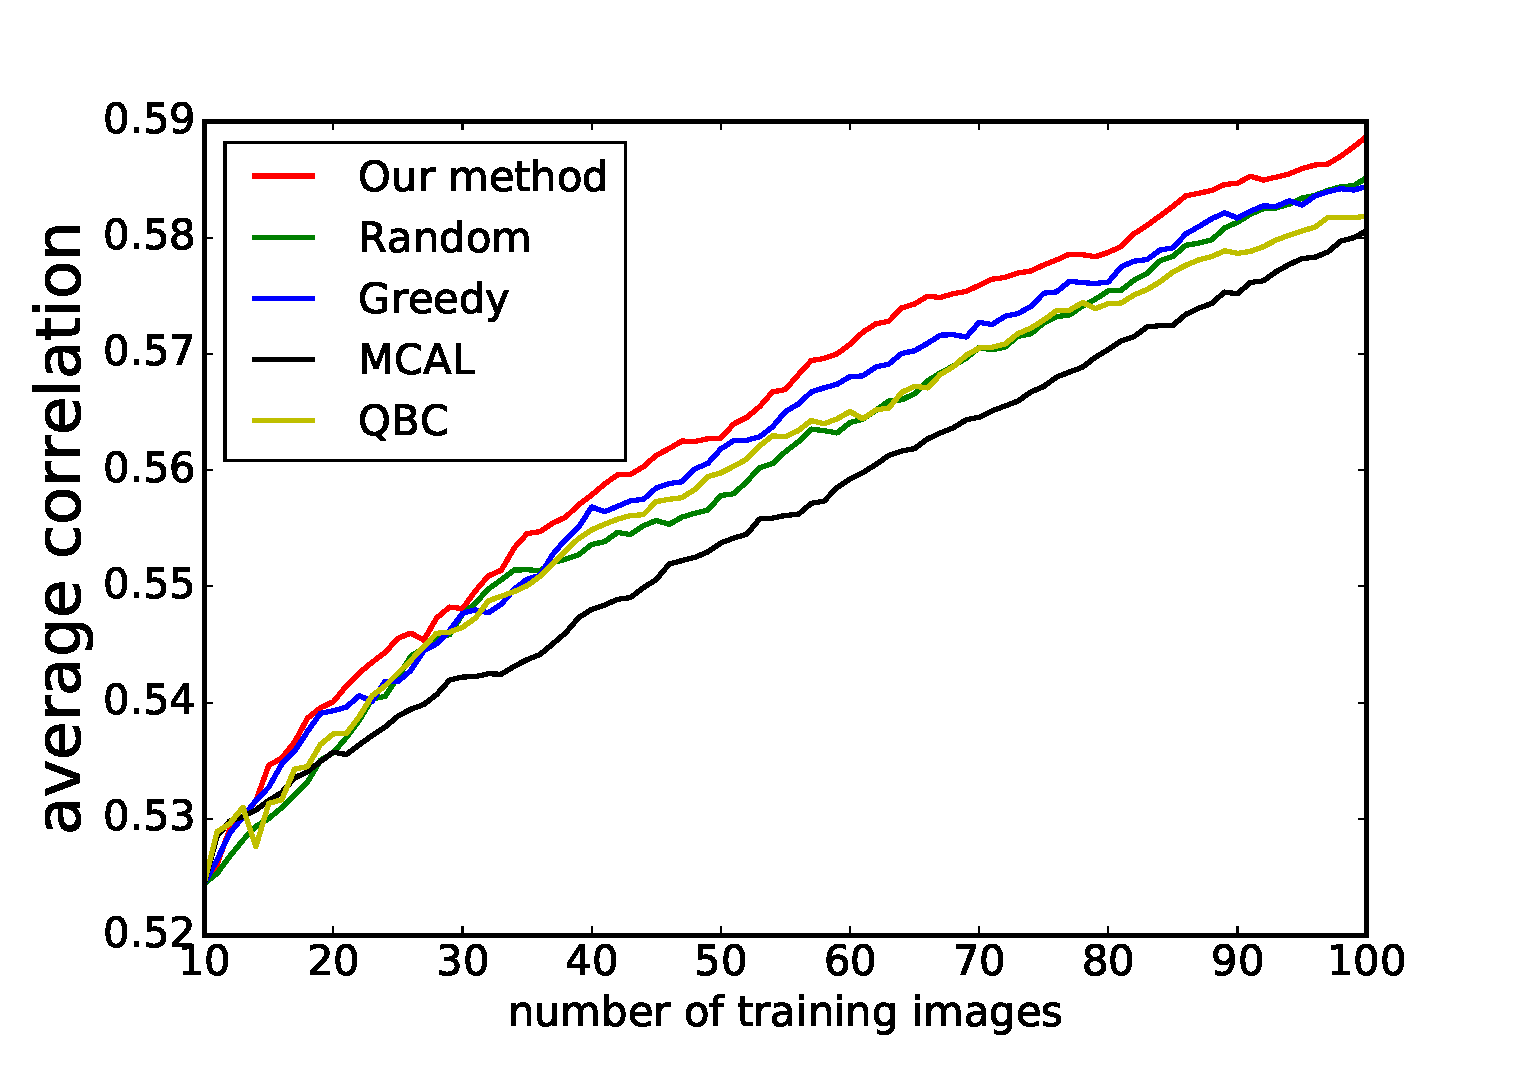
\includegraphics[width=0.5\columnwidth]{figures/UADallTest}\label{6c}
}
\subfloat[Results on REAL-CUR.]{
  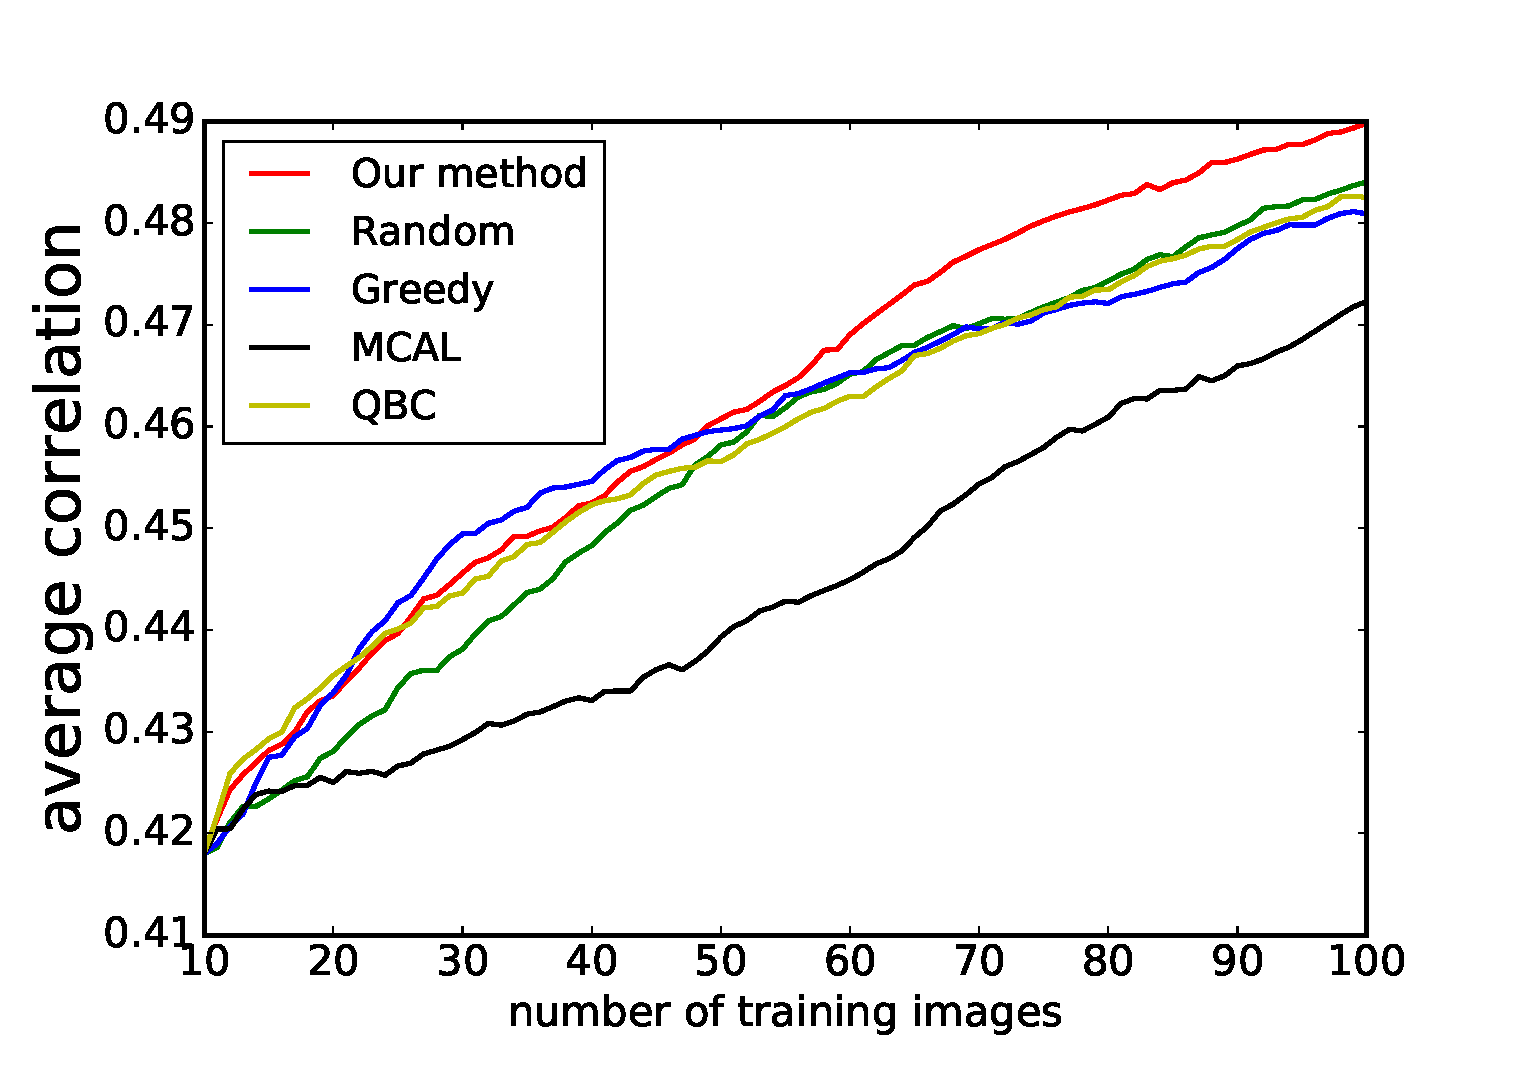
\includegraphics[width=0.5\columnwidth]{figures/RealallTest}\label{6d}
}
\end{center}
\vspace{-0.1in}
\caption{Evaluation of active learning approaches on (a) FLICKR-AES and (b) REAL-CUR on all the images in the photo album.
\vspace{-0.1in}
\label{fig:testresults}}
\end{figure}
%****************************************************************
%**************Different Dataset*********************************
\begin{figure}
\begin{center}
\subfloat[Results on FLICKR-AES]{
  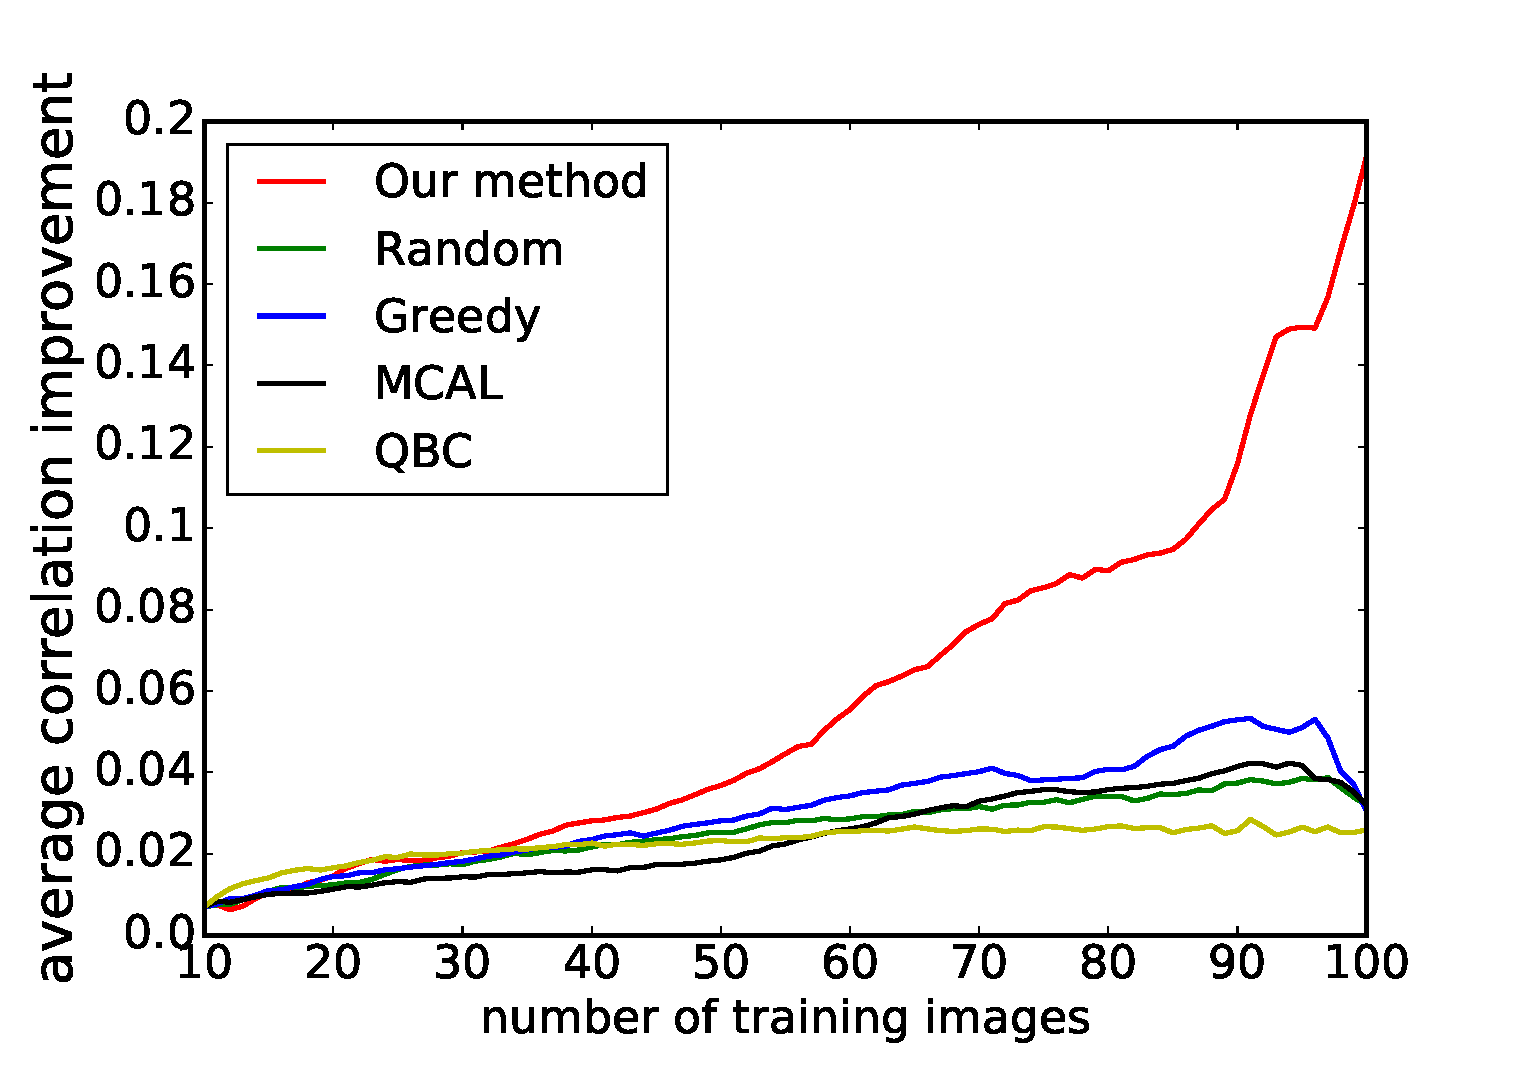
\includegraphics[width=0.5\columnwidth]{figures/methodCompare}\label{6a}
}%\\
\subfloat[Results on REAL-CUR]{
  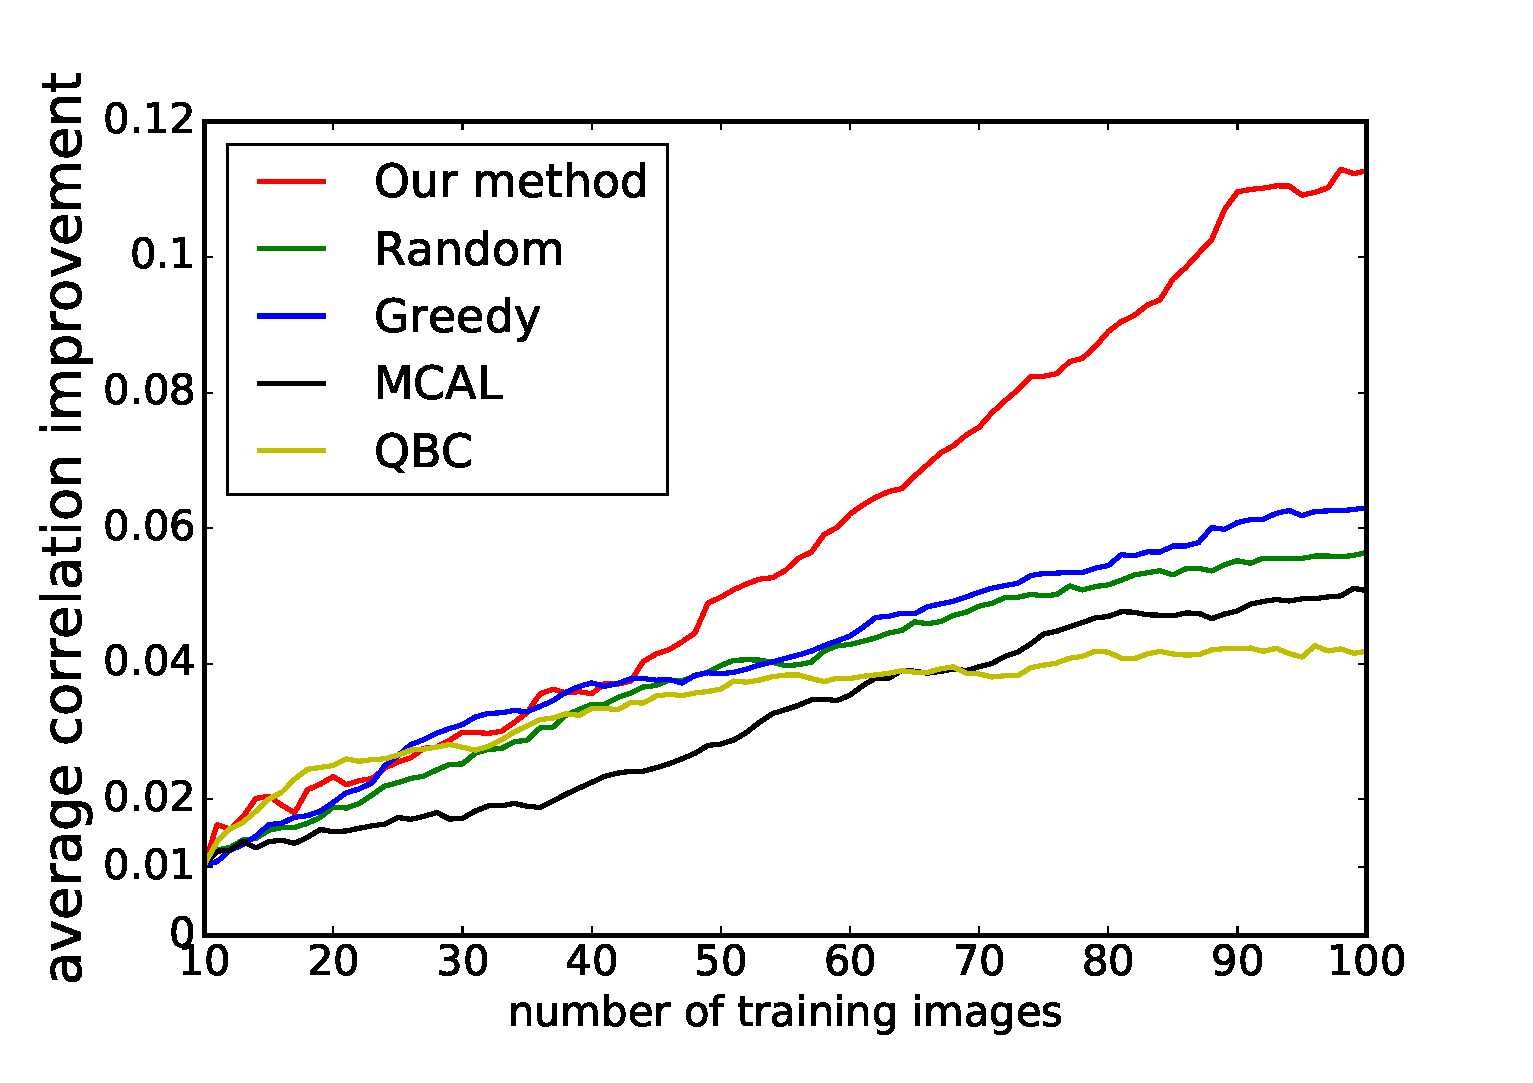
\includegraphics[width=0.5\columnwidth]{figures/realuser}\label{6b}
}
\end{center}
\vspace{-0.1in}
\caption{Evaluation of active learning approaches on (a) FLICKR-AES and (b) REAL-CUR on unseen images in the photo album. 
\vspace{-0.15in}
\label{fig:testresults2}}
\end{figure}
%****************************************************************


\section{Conclusion}
In this work, we address the problem of personalized image aesthetics, and introduce two new datasets to facilitate investigatio of this problem. We  propose a novel residual-based personalized aesthetics model for accommodating individual aesthetics taste with limited annotated examples. We also find that the attributes and contents are both important information for studying individual aesthetics preference. Furthermore, we introduce a new active learning method to interactively select training images and improve the training efficiency and performance of the personalized aesthetics model. One interesting future research direction is to investigate additional cues such as content redundancy, image quality or face recognition for improving user experience in real-world applications.

\endgroup
%******************************************************************************
%******************************************************************************


{\small
\bibliographystyle{ieee}
\bibliography{egbib}
}

\end{document}
